\clearpage % Rozdziały zaczynamy od nowej strony.

\section{Analiza wymagań systemu}

Przed rozpoczęciem implementacji systemu należy go przeanalizować pod kątem wymagań funkcjonalnych oraz niefunkcjonalnych. Twórca powinien uprzednio poznać występujące rodzaje danych, udostępniane na nich operacje oraz klasy użytkowników.

W systemach o architekturze mikroserwisowej należy również odpowiednio wydzielić serwisy, stanowiące spójną całość.

W tym rozdziale zostaną też przedstawione najważniejsze terminy i pojęcia używane w aplikacji, jej wymagania oraz przypadki użycia.

\subsection{Słownik dziedziny problemu}

Słownik najważniejszych pojęć występujących w dziedzinie systemu. W nawiasach podano ich angielskie odpowiedniki, ponieważ w takiej formie zostały one użyte w kodzie aplikacji.

\begin{itemize}

    \item \textbf{Użytkownik zamawiający} (ang. \textit{Ordering User}) - XXX
    \item \textbf{Restauracja} (ang. \textit{Restaurant}) - XXX
    \item \textbf{Kurier} (ang. \textit{Courier}) - XXX
    \item \textbf{Dostawa} (ang. \textit{Order Delivery}) - XXX
    \item \textbf{Zamówienie} (ang. \textit{Order}) - XXX
    \item \textbf{Faktura} (ang. \textit{Invoice}) - XXX
    \item \textbf{Płatność} (ang. \textit{Order Payment}) - XXX
    \item \textbf{Odbiora płatności} (ang. \textit{Payee}) - XXX
    \item \textbf{Płatnik} (ang. \textit{Payer}) - XXX
    \item \textbf{Zamówienie restauracyjne} (ang. \textit{Restaurant Order}) - XXX

\end{itemize}

\subsection{Burza Zdarzeń}

Aby móc podzielić system informatyczny na komponenty, później przekształcone w mikroserwisy, można zastosować np. technikę Burzy Zdarzeń (ang. Event Storming).

Burza Zdarzeń to metoda warsztatowa używana w projektowaniu i analizie systemów opartych na mikroserwisach. Została opracowana przez Alberto Brandoliniego i polega na interaktywnym modelowaniu procesów biznesowych poprzez identyfikację i dyskusję na temat "zdarzeń" mających znaczenie biznesowe. Uczestnicy, wykorzystując kolorowe karteczki, reprezentują różne aspekty systemu, takie jak wydarzenia, komendy, czy modele danych. Ta metoda sprzyja współpracy między różnymi zespołami, pomagając im lepiej zrozumieć procesy biznesowe i technologiczne oraz identyfikować potencjalne problemy i możliwości dla architektury mikroserwisowej.

\begin{figure}[!h]
    \centering 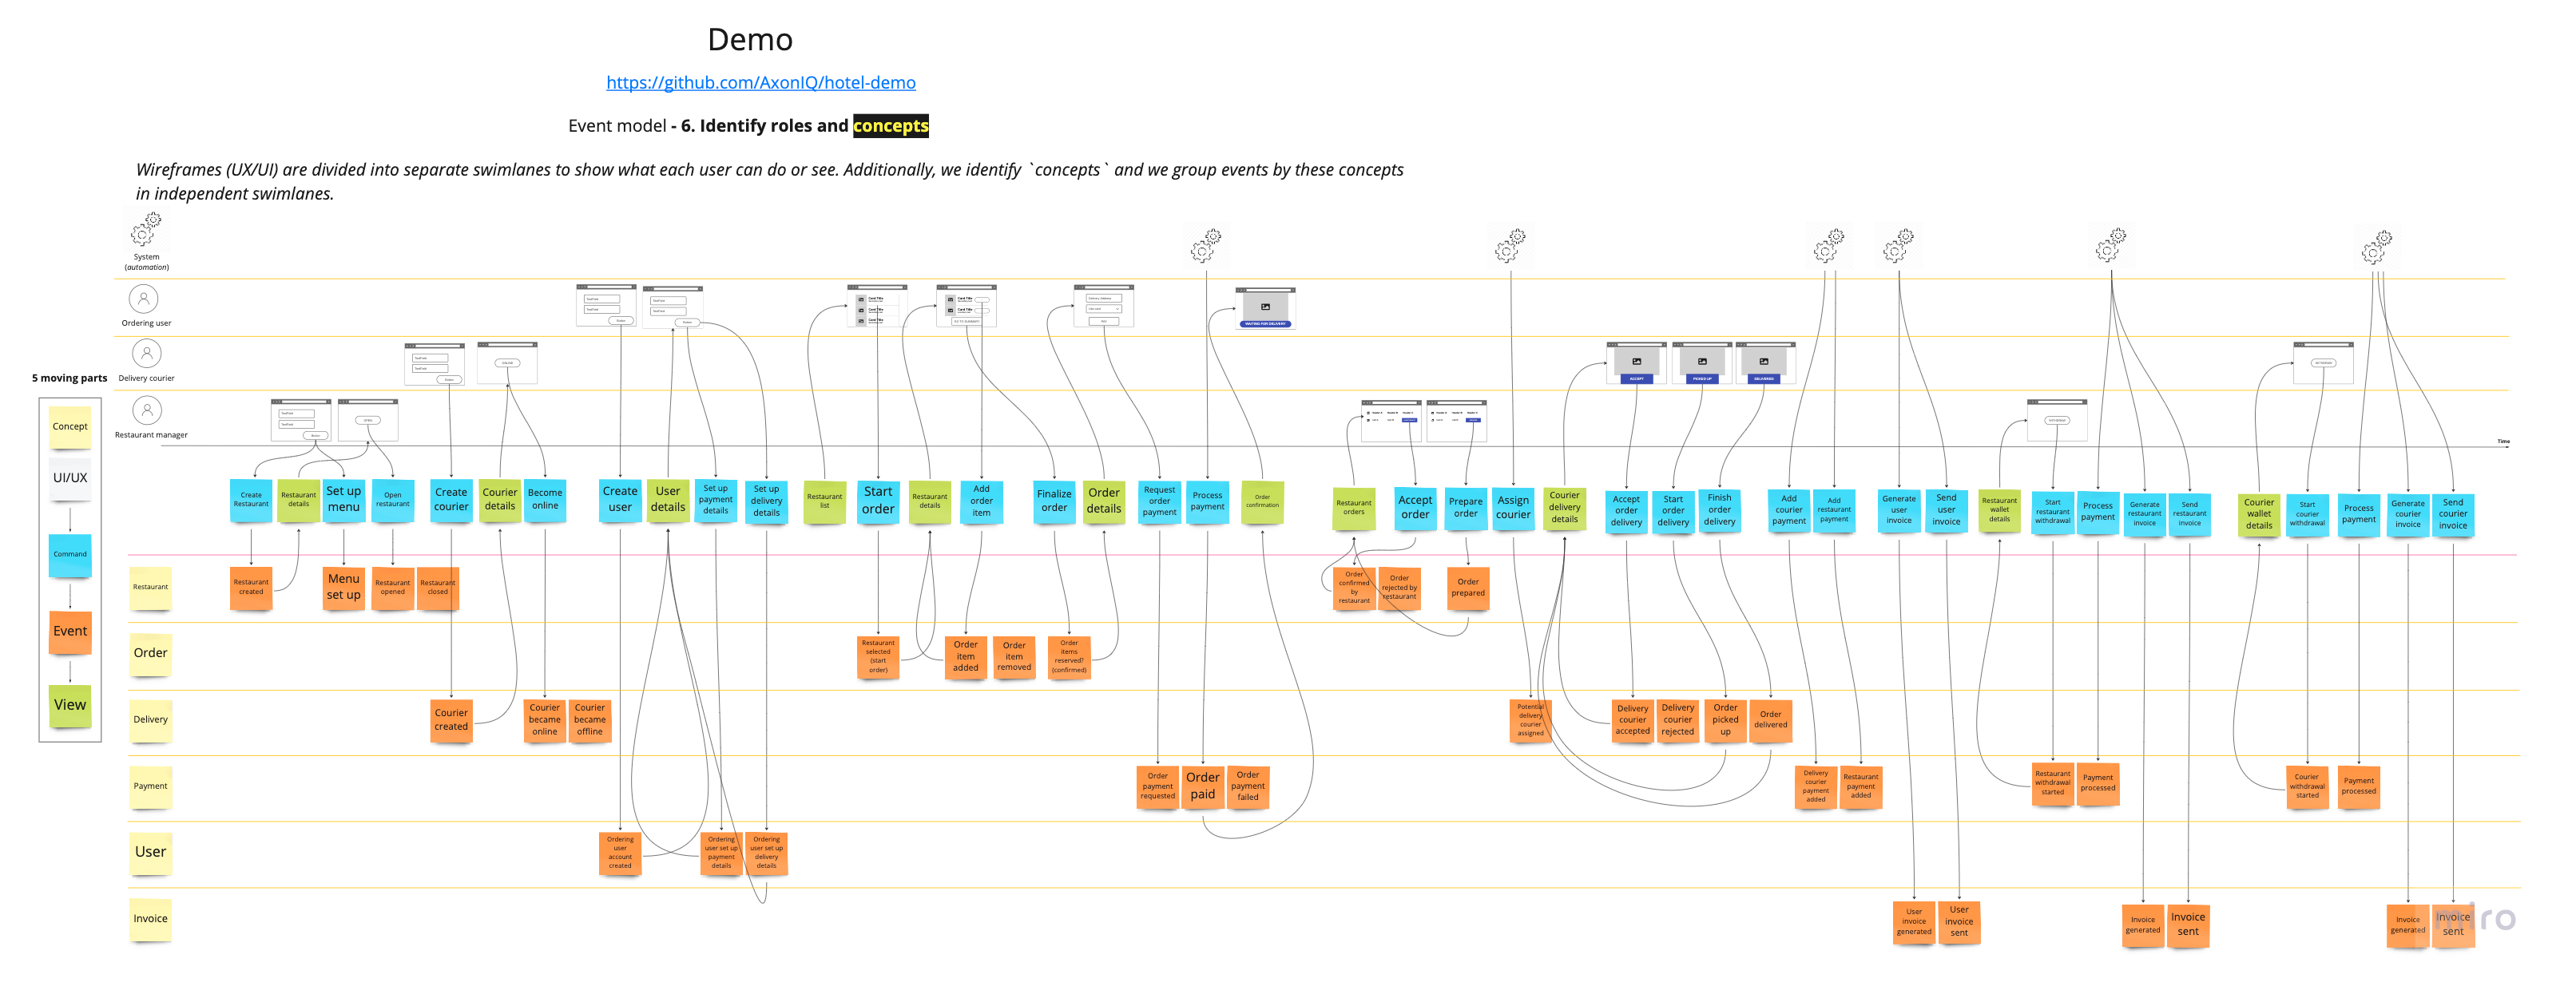
\includegraphics[width=0.8\linewidth]{event_storming.png}
    \caption{Rezultat sesji Burzy Zdarzeń \cite{event_storming_rys}}
\end{figure}


Rezultatem sesji Burzy Zdarzeń powinna być lista zdarzeń zgrupowanych w ramach tzw. agregatów dziedzinowych, czyli obiektów realizujących konkretny zbiór logiki biznesowej. W tej postaci łatwo postawić granice między słabo powiązanymi grupami agregatów. Zbiór agregatów po jednej stronie granicy nazywamy Ograniczonym Kontekstem (ang. Bounded Context). Są to kandydaci do wydzielenia jako mikroserwisy modelowanej aplikacji.

W niniejszym rozdziale przedstawione zostaną wyniki sesji Event Stormingu, która została przeprowadzona z wykorzystaniem narzędzia Miro.

TODO opisac wiecej

Miro \cite{miro} to interaktywna platforma webowa, umożliwiająca tworzenie tablic z notatkami, rysunkami i diagramami. Wybór tego narzędzia był podyktowany jego prostotą użytkowania oraz możliwościami wizualizacji efektów.

\subsection{Identyfikacja Ograniczonych Kontekstów}

W wyniku sesji Event Stormingu zidentyfikowano pięć kontekstów granicznych (Bounded Context \cite{boundedcontext}), które będą kluczowe dla tworzonej aplikacji. Są to:

\textbf{Restaurant} (\textit{Restauracja}) - obejmuje zarządzanie restauracjami, menu oraz definicją i dostępnością produktów,

\textbf{Order} (\textit{Zamówienie}) - odpowiada za proces zamówienia, jego składanie, modyfikowanie, anulowanie oraz koordynuje cały proces przygotowania zamówienia do momentu dostawy,

\textbf{Delivery} (\textit{Dostawa}) - koncentruje się na logistyce dostaw, monitorowaniu statusu dostawy oraz komunikacji z dostawcą. Zarządza również bazą dostawców,

\textbf{Payment} (\textit{Płatność}) - zarządza procesem płatności, obejmuje różne metody płatności oraz obsługę transakcji. Obsługuje wszelkie rozliczenia w ramach systemu,

\textbf{Invoice} (\textit{Faktura}) - odpowiada za generowanie faktur i rachunków dla użytkowników, restauracji oraz dostawców.

TODO

Wymagania funkcjonalne i niefunkcjonalne zostały zidentyfikowane podczas analizy przeprowadzonej w trakcie sesji Event Stormingu.

\subsection{Wymagania funkcjonalne}

\textbf{Jako administrator systemu}
\begin{itemize}
    \item mogę dodać nową restaurację i jej managera.
\end{itemize}

\textbf{Jako manager restauracji}
\begin{itemize}
    \item mogę zaktualizować jej detale,
    \item mogę dodać nowe menu,
    \item mogę zaktualizować jej dostępność (otwarta/zamknięta),
    \item mogę przyjąć albo odrzucić zamówienie,
    \item mogę zaktualizować status zamówienia,
    \item mogę wypłacić środki za zamówienia i otrzymać fakturę.
\end{itemize}

\textbf{Jako dostawca}
\begin{itemize}
    \item mogę zarejestrować się w systemie,
    \item mogę zaktualizować swój status (dostępny/niedostępny),
    \item mogę przyjąć albo odrzucić zamówienie,
    \item mogę zaktualizować status dostawy,
    \item mogę wypłacić środki za dostarczone zamówienia i otrzymać fakturę.
\end{itemize}

\textbf{Jako zamawiający}
\begin{itemize}
    \item mogę zarejestrować się w systemie,
    \item mogę dodać metodę płatności,
    \item mogę dodać detale dostawy,
    \item mogę rozpocząć proces zamówienia wybierając restaurację,
    \item mogę wybrać dania z menu,
    \item mogę złożyć zamówienie,
    \item mogę opłacić zamówienie,
    \item mogę podejrzeć status zamówienia,
    \item mogę otrzymać fakturę za zamówienie.
\end{itemize}

TODO

\subsection{Przypadki użycia}

XXX

\subsection{Wymagania niefunkcjonalne}

\textbf{Skalowalność} - każdy z komponentów systemu powinien być skalowalny w zależności od obciążenia. Każdy mikroserwis powinien móc być replikowany.

\textbf{Wysoka dostępność} - jeżeli jeden mikroserwis nie jest dostępny, inne mikroserwisy powinny nadal działać poprawnie.

\textbf{Bezpieczeństwo} - aplikacja powinna zapewniać odpowiednie zabezpieczenia w celu ochrony poufności, integralności i dostępności danych. Dostęp do mikroserwisów powinien być chroniony przez autoryzację i uwierzytelnianie, a dane powinny być szyfrowane w tranzycie.

\textbf{Monitorowanie i logowanie} - aplikacja powinna umożliwiać monitorowanie i logowanie zdarzeń w celu analizy i debugowania. Każdy mikroserwis powinien logować swoje zdarzenia w centralnym repozytorium, a system powinien umożliwiać monitorowanie stanu mikroserwisów.

\textbf{Wydajność} - system powinien umożliwiać równoległe przetwarzanie minimum 10 dowolnych żądań na sekundę.

\textbf{Synchronizacja i spójność danych} - system powinien zapewniać spójność danych pomiędzy mikroserwisami.
    
\textbf{Testowalność} - system powinien być łatwy do testowania, zarówno jednostkowo jak i integracyjnie.

TODO